%----------------------------------------------------------------------------------------
%	PART - Conversing with Your X16
%----------------------------------------------------------------------------------------

\makeatletter\@openrightfalse
\part{Conversing with Your X16}

\chaptertypein{
	\keybackgroundcolor{gray}
	\keytextcolor{black}
	10 PRINT "WHAT IS YOUR NAME?"\\
	20 INPUT N\$\\
	30 PRINT\\
	40 PRINT "HELLO, "; N\$; "!"\\
	50 PRINT "NICE TO MEET YOU!"
}

\begin{tikzpicture}
	\hyphenpenalty=10000
	\bubble{2.5in}{2.6in}{5.2}{6.6}{
		This line asks you a question by printing it to the screen.}
	\bubble{2.5in}{1.9in}{4.0}{5.6}{
		This line waits for you to type something and remembers it as N\$.}
	\bubble{2.5in}{1.2in}{5.5}{3.5}{
		These lines greet you by name!}
\end{tikzpicture}

%----------------------------------------------------------------------------------------
%	CHAPTER - Conversing with Your X16
%----------------------------------------------------------------------------------------

\chapter*{Conversing with Your X16}\index{INPUT}\index{Variables}
\addcontentsline{toc}{chapter}{\protect\numberline{}Conversing with Your X16}

Good morning, Commander X16!  Your mission (and we know you are going to accept
it) is to respond to us whenever we touch just a few keys!

Yes, your X16 is ready, able, and willing to respond to your touch.  So let's
buckle down to some non-stop fun!

So far, your programs have just displayed information to the screen.  But what
if you want your program to ask questions and respond to your answers?  In this
chapter, you'll learn how to have a real conversation with your Commander X16!

%----------------------------------------------------------------------------------------
%	SECTION - What's Your Name?
%----------------------------------------------------------------------------------------

\section{What's Your Name?}\index{INPUT}

Let's type in the program from the beginning of this chapter and see what
happens.  Clear the screen by holding down the \shiftkey key and pressing the
\clrhomekey key.  Then type {\ttfamily NEW} and press \returnkey to start fresh.

Now type in the program exactly as shown:

\codeblock{
	10 PRINT "WHAT IS YOUR NAME?"\\
	20 INPUT N\$\\
	30 PRINT\\
	40 PRINT "HELLO, "; N\$; "!"\\
	50 PRINT "NICE TO MEET YOU!"\\
}

\reminder{
	Don't forget to press \returnkey at the end of each line!
}

When you've finished typing, type {\ttfamily RUN} and press \returnkey.  The
X16 responds:

\begin{center}
\screenbox{3in}{1.5in}{
	WHAT IS YOUR NAME?\\
	? \cursor
}
\end{center}

\begin{tikzpicture}
	\hyphenpenalty=10000
	\smallbubble{3.0in}{0.8in}{4.8}{2.85}{
		Notice that the computer automatically adds the question mark (?) to
		show you that it's waiting for an input.}
\end{tikzpicture}

\vspace{16pt}

The X16 is waiting for you!  Type your name (or any name you like) and press
\returnkey.  If your name happens to be {\ttfamily ALEX}, you might type:

\keybackgroundcolor{white}
\keytextcolor{black}
\key{a} \key{l} \key{e} \key{x} \returnkey\\

And whoopee!  Your name appears on the screen with a friendly greeting!

\begin{center}
\screenbox{3in}{2in}{
	WHAT IS YOUR NAME?\\
	? ALEX\\\\
	HELLO, ALEX!\\
	NICE TO MEET YOU!\\\\
	READY.\\
	\cursor
}
\end{center}

To ask for another name, just type {\ttfamily RUN} again and you will see the
same \emph{prompt} asking for your name.  A prompt is a question directed to
you in an effort to get information into the X16.

%----------------------------------------------------------------------------------------
%	SECTION - The INPUT Statement
%----------------------------------------------------------------------------------------

\section{The INPUT Statement}\index{INPUT}

The {\ttfamily INPUT} statement is one of the most useful ways for your program
to collect information from you through the keyboard.  Let's go through the
steps of our program to understand what we told the X16 to do.

\codeblock{
	10 PRINT "WHAT IS YOUR NAME?"\\
}

Line 10 displays the message {\ttfamily WHAT IS YOUR NAME?} on the screen.
This is our prompt---the question we want to ask.

\codeblock{
	20 INPUT N\$\\
}

Line 20 is where the magic happens!  The {\ttfamily INPUT} statement tells the
X16 to:

\begin{enumerate}
	\item Print a question mark ({\ttfamily ?}) to let you know it's waiting
	\item Wait for you to type something and press \returnkey
	\item Take whatever you typed and store it in a \emph{variable} called
		{\ttfamily N\$}
\end{enumerate}

In our example, when you typed {\ttfamily ALEX}, the X16 stored the word
{\ttfamily ALEX} inside {\ttfamily N\$}.  This is a kind of shorthand for the
computer---wherever you use {\ttfamily N\$} in your program, the X16 will
remember that it means {\ttfamily ALEX}.

\codeblock{
	30 PRINT\\
}

Line 30 simply prints a blank line to make our output look nicer.

\codeblock{
	40 PRINT "HELLO, "; N\$; "!"\\
	50 PRINT "NICE TO MEET YOU!"\\
}

Lines 40 and 50 print the greeting.  Notice how line 40 combines the word
{\ttfamily HELLO,} with whatever was stored in {\ttfamily N\$}, followed by an
exclamation mark.  The semicolons ({\ttfamily ;}) tell the X16 to print
everything on the same line without any extra spaces.

\tip{Prompts in INPUT}{

	You can combine the prompt and the {\ttfamily INPUT} statement on one line!
	Instead of using two lines like this:\\

	\codeblock{
		10 PRINT "WHAT IS YOUR NAME?"\\
		20 INPUT N\$\\
	}

	You can write it as a single line:\\

	\codeblock{
		10 INPUT "WHAT IS YOUR NAME"; N\$\\
	}

	This prints your prompt, then the question mark, and waits for input---all
	in one statement!

}

%----------------------------------------------------------------------------------------
%	SECTION - Introducing Variables
%----------------------------------------------------------------------------------------

\section{Introducing Variables}\index{Variables}

You've just used something called a \emph{variable}.  Variables are one of the
most powerful features of any programming language.  Understanding how
variables work will open up a whole new world of possibilities for your
programs.

Imagine a number of boxes inside the computer that can hold information.  Each
box has a label---a name that you choose.  That name is the variable, and it
represents whatever information is stored in its box.

\begin{center}
\screenbox{2.5in}{1in}{
	N\$ \hspace{0.5in} ALEX\\\\
	X \hspace{0.65in} 42\\\\
	A\$ \hspace{0.5in} HELLO WORLD\\
}
\end{center}

\begin{tikzpicture}
	\hyphenpenalty=10000
	\tinybubble{3.0in}{1.4in}{4.5}{3.3}{
		Each variable is like a labeled box holding a value.}
\end{tikzpicture}

\vspace{16pt}

\subsection{String Variables}

The variable {\ttfamily N\$} that we used is called a \emph{string variable}.
The dollar sign ({\ttfamily \$}) at the end tells the X16 that this variable
will hold text---letters, numbers, symbols, or any characters you can type.
Text stored in a variable is called a \emph{string} because it's a string of
characters all linked together.

Here are some examples of string variables:

\codeblock{
	N\$ = "ALEX"\\
	CITY\$ = "NEW YORK"\\
	MSG\$ = "HELLO WORLD!"\\
}

\tryit{

	Try this in direct mode (without line numbers).  Type each line and press
	\returnkey:\\

	\codeblock{
		A\$ = "COMMANDER"\\
		B\$ = "X16"\\
		PRINT A\$; " "; B\$\\
	}

	What happens?  The X16 prints the contents of both variables with a space
	between them!

}

\subsection{Numeric Variables}

Not all variables hold text.  \emph{Numeric variables} hold numbers and don't
have a dollar sign at the end.  You can use these for counting, calculating,
and keeping score in games.

\codeblock{
	X = 10\\
	Y = 25\\
	SCORE = 1000\\
}

Try this quick experiment:

\codeblock{
	X = 10\\
	Y = 25\\
	PRINT X + Y\\
}

The X16 will print {\ttfamily 35}---the sum of the two numbers stored in your
variables!

\subsection{Variable Names}

When choosing names for your variables, keep these rules in mind:

\begin{itemize}
	\item Variable names must start with a letter (A-Z)
	\item They can contain letters and numbers
	\item Only the first two characters matter to the X16, so {\ttfamily SCORE}
		and {\ttfamily SC} refer to the same variable
	\item Add {\ttfamily \$} at the end for string variables
	\item Don't use BASIC keywords like {\ttfamily PRINT} or {\ttfamily GOTO}
		as variable names
\end{itemize}

\note{

	Because only the first two characters of a variable name matter, be careful
	not to accidentally use the same variable twice!  For example, {\ttfamily
	PLAYER} and {\ttfamily POINTS} would both be seen as {\ttfamily PL} by the
	X16.

}

\subsection{Changing Variables}

One of the most powerful things about variables is that you can change their
value at any time.  When you assign a new value, it replaces the old one in the
same box.

This allows you to write statements that might look strange at first:

\codeblock{
	X = X + 1\\
}

This would never work in algebra, but it's one of the most common things you'll
do in programming!  It means: take the current value of {\ttfamily X}, add one
to it, and put the result back into {\ttfamily X}.

\tryit{

	Try this program to see variables change:\\

	\codeblock{
		10 X = 1\\
		20 PRINT "X IS NOW"; X\\
		30 X = X + 1\\
		40 IF X < 6 THEN GOTO 20\\
		50 PRINT "DONE!"\\
	}

	Watch how {\ttfamily X} increases each time through the loop!

}

%----------------------------------------------------------------------------------------
%	SECTION - The GET Statement
%----------------------------------------------------------------------------------------

\section{The GET Statement}\index{GET}

The {\ttfamily INPUT} statement is great when you want someone to type a word
or sentence and press \returnkey.  But what if you only want to read a single
keypress?  That's where {\ttfamily GET} comes in!

{\ttfamily GET} reads one character from the keyboard \emph{without} waiting
for \returnkey.  The moment a key is pressed, your program can respond.

Try this short program:

\codeblock{
	10 GET A\$\\
	20 IF A\$ = "" THEN GOTO 10\\
	30 PRINT A\$;\\
	40 GOTO 10\\
}

\begin{center}
\screenbox{3in}{1.5in}{
	RUN\\
	HELLO X16\cursor
}
\end{center}

\begin{tikzpicture}
	\hyphenpenalty=10000
	\smallbubble{3.0in}{0.8in}{4.5}{2.3}{
		Each key you press appears instantly---no \returnkey needed!}
\end{tikzpicture}

\vspace{16pt}

Type {\ttfamily RUN} and press \returnkey.  Now press any keys and watch them
appear on the screen one at a time!  Press the \runstopkey key to stop the
program.

Let's understand how this works:

\codeblock{
	10 GET A\$\\
}

Line 10 checks the keyboard.  If a key is being pressed, its character goes
into {\ttfamily A\$}.  If no key is pressed, {\ttfamily A\$} becomes empty
(contains nothing).

\codeblock{
	20 IF A\$ = "" THEN GOTO 10\\
}

Line 20 is very important!  Unlike {\ttfamily INPUT}, which waits patiently for
you to type something, {\ttfamily GET} keeps running whether you press a key or
not.  This line checks if {\ttfamily A\$} is empty (the two quotation marks
with nothing between them).  If it is, the program goes back to line 10 to
check again.  This creates a loop that keeps checking until you press
something.

\codeblock{
	30 PRINT A\$;\\
	40 GOTO 10\\
}

Lines 30 and 40 print the character and go back to check for another keypress.

\note{

	Notice that {\ttfamily GET} does not automatically display what you type on
	the screen.  You must {\ttfamily PRINT} it yourself if you want to see it.
	This gives you complete control over what appears on screen.

}

\subsection{Using GET for Menus}

{\ttfamily GET} is perfect for creating menus where the user presses a single
key to make a choice:

\codeblock{
	10 PRINT "CHOOSE AN OPTION:"\\
	20 PRINT "1. SAY HELLO"\\
	30 PRINT "2. SAY GOODBYE"\\
	40 PRINT "3. EXIT"\\
	50 GET A\$: IF A\$ = "" THEN 50\\
	60 IF A\$ = "1" THEN PRINT "HELLO!": GOTO 10\\
	70 IF A\$ = "2" THEN PRINT "GOODBYE!": GOTO 10\\
	80 IF A\$ = "3" THEN END\\
	90 GOTO 50\\
}

Run this program and try pressing 1, 2, or 3.  The program responds instantly
to your keypress!

\tip{Combining Statements}{

	Line 50 shows a useful trick: you can put multiple statements on one line
	by separating them with a colon ({\ttfamily :}).  The line:\\

	\codeblock{
		50 GET A\$: IF A\$ = "" THEN 50\\
	}

	Does two things: gets a keypress, then checks if it was empty.  This is a
	common pattern when using {\ttfamily GET}.

}

%----------------------------------------------------------------------------------------
%	SECTION - A Temperature Converter
%----------------------------------------------------------------------------------------

\section{A Temperature Converter}\index{INPUT}

Now let's put everything together with a useful program!  This temperature
converter shows {\ttfamily INPUT} in action with numeric variables:

\codeblock{
	10 PRINT "TEMPERATURE CONVERTER"\\
	20 PRINT\\
	30 PRINT "ENTER DEGREES FAHRENHEIT:"\\
	40 INPUT F\\
	50 C = (F - 32) * 5 / 9\\
	60 PRINT\\
	70 PRINT F; " DEGREES F ="\\
	80 PRINT C; " DEGREES C"\\
	90 PRINT\\
	100 GOTO 30\\
}

Run the program and enter a temperature in Fahrenheit.  The X16 will calculate
the Celsius equivalent!

\begin{center}
\screenbox{3.25in}{2.5in}{
	TEMPERATURE CONVERTER\\\\
	ENTER DEGREES FAHRENHEIT:\\
	? 32\\\\
	32 DEGREES F =\\
	0 DEGREES C\\\\
	ENTER DEGREES FAHRENHEIT:\\
	? \cursor
}
\end{center}

Notice that line 40 uses {\ttfamily INPUT F} without the dollar sign.  This
tells the X16 to expect a \emph{number}, not text.  The number gets stored in
the numeric variable {\ttfamily F}, which we then use in the calculation on
line 50.

Press the \runstopkey key when you're done converting temperatures.

\tryit{

	Can you modify this program to convert from Celsius to Fahrenheit instead?
	The formula is: F = C * 9 / 5 + 32

}

%----------------------------------------------------------------------------------------
%	SECTION - Choose a Number
%----------------------------------------------------------------------------------------

\section{Choose a Number}

Here's a fun program that combines {\ttfamily INPUT} with a simple guessing
element:

\codeblock{
	10 PRINT "PICK A NUMBER FROM 1 TO 10"\\
	20 INPUT N\\
	30 IF N < 1 OR N > 10 THEN GOTO 10\\
	40 PRINT\\
	50 PRINT "YOU PICKED"; N\\
	60 PRINT "THAT'S A ";\\
	70 IF N < 4 THEN PRINT "LOW": GOTO 100\\
	80 IF N > 7 THEN PRINT "HIGH": GOTO 100\\
	90 PRINT "MIDDLE"\\
	100 PRINT "NUMBER!"\\
}

This program asks you to pick a number between 1 and 10.  Line 30 makes sure
you entered a valid number---if not, it asks again.  Then it tells you whether
your number is low, middle, or high!

%----------------------------------------------------------------------------------------
%	SECTION - What You've Learned
%----------------------------------------------------------------------------------------

\section{What You've Learned}

Congratulations!  You've discovered how to make your Commander X16 truly
interactive.  In this chapter, you learned:

\begin{itemize}

	\item The {\ttfamily INPUT} statement lets your program ask questions and
		wait for answers

	\item \emph{Variables} are like labeled boxes that store information

	\item \emph{String variables} (with {\ttfamily \$}) hold text, while
		\emph{numeric variables} hold numbers

	\item The {\ttfamily GET} statement reads a single keypress instantly,
		without waiting for \returnkey

	\item You can create menus, calculators, and all sorts of interactive
		programs!

\end{itemize}

\vspace{16pt}

Now that you can have a conversation with your X16, you're ready to create
programs that respond to the user in all sorts of interesting ways.  Try
combining what you learned here with the graphics and sound from earlier
chapters to make your programs come alive!

\@openrighttrue\makeatother
